\documentclass[10pt]{article}
\usepackage[polish]{babel}
\usepackage[utf8]{inputenc}
\usepackage[T1]{fontenc}
\usepackage{amsmath}
\usepackage{amsfonts}
\usepackage{amssymb}
\usepackage[version=4]{mhchem}
\usepackage{stmaryrd}
\usepackage{graphicx}
\usepackage[export]{adjustbox}
\graphicspath{ {./images/} }
\usepackage{bbold}

%New command to display footnote whose markers will always be hidden
\let\svthefootnote\thefootnote
\newcommand\blfootnotetext[1]{%
  \let\thefootnote\relax\footnote{#1}%
  \addtocounter{footnote}{-1}%
  \let\thefootnote\svthefootnote%
}

%Overriding the \footnotetext command to hide the marker if its value is `0`
\let\svfootnotetext\footnotetext
\renewcommand\footnotetext[2][?]{%
  \if\relax#1\relax%
    \ifnum\value{footnote}=0\blfootnotetext{#2}\else\svfootnotetext{#2}\fi%
  \else%
    \if?#1\ifnum\value{footnote}=0\blfootnotetext{#2}\else\svfootnotetext{#2}\fi%
    \else\svfootnotetext[#1]{#2}\fi%
  \fi
}

\newcommand\Varangle{\mathop{{<\!\!\!\!\!\text{\small)}}\:}\nolimits}

\begin{document}
\section*{CENTRALNA \\
 KOMISJA \\
 EGZAMINACYJNA}
\begin{center}
\begin{tabular}{|l|l|}
\hline
Rodzaj dokumentu: & \begin{tabular}{l}
Zasady Oceniania rozwiązań \\
zadań \\
\end{tabular} \\
\hline
Egzamin: & Egzamin maturalny \\
\hline
Przedmiot: & Matematyka \\
\hline
Poziom: & Poziom rozszerzony \\
\hline
Formy arkusza: & \begin{tabular}{l}
EMAP-R0-100, EMAP-R0-200, \\
EMAP-R0-300, EMAP-R0-400,, \\
EMAP-R0-K00, EMAP-R0-700, EMAP-R0-Q00,, \\
EMAU-R0-100 \\
\end{tabular} \\
\hline
Termin egzaminu: & 15 maja 2024 r. \\
\hline
\begin{tabular}{l}
Data publikacji \\
dokumentu: \\
\end{tabular} & 28 czerwca 2024 r. \\
\hline
\end{tabular}
\end{center}

\section*{ZADANIA ZAMKNIETE}
\section*{Zadanie 1. (0-1)}
\begin{center}
\begin{tabular}{|l|l|}
\hline
\multicolumn{2}{|c|}{Wymagania egzaminacyjne 2024 ${ }^{1}$} \\
\hline
\multicolumn{1}{|c|}{Wymaganie ogólne} & \multicolumn{1}{c|}{Wymaganie szczegółowe $^{|c|}$} \\
\hline
II. Wykorzystanie i interpretowanie & Zdający: \\
reprezentacji. & 8.1R) oblicza odległość punktu od prostej. \\
\hline
\end{tabular}
\end{center}

\section*{Zasady oceniania}
1 pkt - odpowiedź poprawna.\\
0 pkt - odpowiedź niepoprawna albo brak odpowiedzi.

\section*{Rozwiązanie}
A

Zadanie 2. (0-1)

\begin{center}
\begin{tabular}{|l|l|}
\hline
\multicolumn{2}{|c|}{Wymagania egzaminacyjne 2024} \\
\hline
\multicolumn{1}{|c|}{Wymaganie ogólne} & \multicolumn{1}{c|}{Wymaganie szczegółowe} \\
\hline
II. Wykorzystanie i interpretowanie & Zdający: \\
reprezentacji. & 3.8R) rozwiązuje równania i nierówności \\
 & z wartością bezwzględną [...]. \\
\hline
\end{tabular}
\end{center}

\section*{Zasady oceniania}
1 pkt - odpowiedź poprawna.\\
0 pkt - odpowiedź niepoprawna albo brak odpowiedzi.

\section*{Rozwiązanie}
B

\footnotetext{${ }^{1}$ Rozporządzenie Ministra Edukacji i Nauki z dnia 1 sierpnia 2022 r. w sprawie wymagań egzaminacyjnych dla egzaminu maturalnego przeprowadzanego w roku szkolnym 2022/2023 i 2023/2024 (Dz.U. poz. 1698).
}\section*{Zadanie 3. (0-1)}
\begin{center}
\begin{tabular}{|l|l|}
\hline
\multicolumn{2}{|c|}{Wymagania egzaminacyjne 2024} \\
\hline
\multicolumn{1}{|c|}{Wymaganie ogólne} & \multicolumn{1}{c|}{Wymaganie szczegółowe} \\
\hline
I. Wykorzystanie i tworzenie informacji. & Zdający: \\
 & 4.2R) szkicuje wykres funkcji określonej \\
 & w różnych przedziałach różnymi wzorami; \\
 & odczytuje własności takiej funkcji z wykresu. \\
\hline
\end{tabular}
\end{center}

\section*{Zasady oceniania}
1 pkt - odpowiedź poprawna.\\
0 pkt - odpowiedź niepoprawna albo brak odpowiedzi.

\section*{Rozwiązanie}
B

Zadanie 4. (0-1)

\begin{center}
\begin{tabular}{|l|l|}
\hline
\multicolumn{2}{|c|}{Wymagania egzaminacyjne 2024} \\
\hline
\multicolumn{1}{|c|}{Wymaganie ogólne} & \multicolumn{1}{c|}{Wymaganie szczegółowe} \\
\hline
II. Wykorzystanie i interpretowanie & Zdający: \\
reprezentacji. & 11.1R) oblicza granice funkcji [...]. \\
\hline
\end{tabular}
\end{center}

\section*{Zasady oceniania}
1 pkt - odpowiedź poprawna.\\
0 pkt - odpowiedź niepoprawna albo brak odpowiedzi.

\section*{Rozwiązanie}
C

\section*{ZadAnie otwarte (kodowane)}
\section*{Zadanie 5. (0-2)}
\begin{center}
\begin{tabular}{|l|l|}
\hline
\multicolumn{2}{|c|}{Wymagania egzaminacyjne 2024} \\
\hline
\multicolumn{1}{|c|}{Wymaganie ogólne} & \multicolumn{1}{c|}{Wymaganie szczegółowe} \\
\hline
II. Wykorzystanie i interpretowanie & Zdajacy: \\
reprezentacji. & $2.2 \mathrm{R})$ dzieli wielomiany przez dwumian \\
 & $a x+b$. \\
\hline
\end{tabular}
\end{center}

\section*{Zasady oceniania}
2 pkt - odpowiedź całkowicie poprawna.\\
0 pkt - odpowiedź niepełna lub niepoprawna albo brak odpowiedzi.

\section*{Rozwiązanie}
\begin{center}
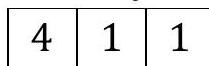
\includegraphics[max width=\textwidth]{2025_02_07_d8b842ccd39861fafa8ag-04}
\end{center}

\section*{ZADANIA OTWARTE (NIEKODOWANE)}
\section*{Uwagi ogólne:}
\begin{enumerate}
  \item Akceptowane są wszystkie rozwiązania merytorycznie poprawne i spełniające warunki zadania.
  \item Jeżeli zdający popełni błędy rachunkowe, które na żadnym etapie rozwiązania nie upraszczają i nie zmieniają danego zagadnienia, lecz stosuje poprawną metodę i konsekwentnie do popełnionych błędów rachunkowych rozwiązuje zadanie, to może otrzymać co najwyżej ( $n-1$ ) punktów (gdzie $n$ jest maksymalną możliwą do uzyskania liczbą punktów za dane zadanie).
\end{enumerate}

\section*{Zadanie 6. (0-3)}
\begin{center}
\begin{tabular}{|l|l|}
\hline
\multicolumn{2}{|c|}{Wymagania egzaminacyjne 2024} \\
\hline
\multicolumn{1}{|c|}{Wymaganie ogólne} & \multicolumn{1}{c|}{Wymaganie szczegółowe} \\
\hline
V. Rozumowanie i argumentacja. & Zdający: \\
 & 1.2R) stosuje w obliczeniach wzór na \\
 & logarytm potęgi oraz wzór na zamianę \\
 & podstawy logarytmu. \\
\hline
\end{tabular}
\end{center}

\section*{Zasady oceniania}
3 pkt - przeprowadzenie pełnego rozumowania.\\
2 pkt - przekształcenie wyrażenia $\frac{2 \log _{5} 4+\log _{4} 3}{\log _{5} 4 \cdot\left(1+\log _{4} 3\right)}$ lub $\log _{12} 80$, lub obydwu tych wyrażeń do takiej postaci, z której poprzez jednokrotne zastosowanie wzoru na\\
logarytm iloczynu lub wzoru na zamianę podstawy logarytmu, lub logarytmu potęgi oraz ewentualne kilkukrotne przekształcenie wyrażenia wymiernego można otrzymać teze\\
ALBO

\begin{itemize}
  \item zapisanie jednego równania wymiernego z $a, b$ oraz niewiadomą $x, \mathrm{np}$. $b x+x=\frac{1}{a}+2$ (dla sposobu III),\\
ALBO
  \item zapisanie liczby 5 w postaci $4^{\frac{1}{a}}$ oraz liczby 4 w postaci $12^{\frac{1}{1+b}}$ (dla sposobu IV).
\end{itemize}

1 pkt - zastosowanie wzoru na zamianę podstawy logarytmu lub na logarytm iloczynu, np.

$$
\begin{aligned}
& \log _{12} 80=\frac{\log _{4} 80}{\log _{4} 12}, \log _{12} 80=\frac{\log _{5} 80}{\log _{5} 12}, 2 \cdot \log _{5} 4+1=\log _{5}(4 \cdot 4 \cdot 5) \\
& 1+\log _{4} 3=\log _{4}(4 \cdot 3) \\
& A L B O
\end{aligned}
$$

\begin{itemize}
  \item zapisanie dwóch spośród liczb 3, 4, 5 jako potęgi, której podstawą jest trzecia z nich, a wykładnik jest zależny od $a$ lub $b$, np.: $5=4^{\frac{1}{a}}$ i $3=4^{b}$ oraz zapisanie równania $12^{x}=80$ (dla sposobu III),\\
ALBO
  \item zapisanie liczby 4 w postaci $12^{\frac{1}{1+b}}$ (dla sposobu IV).
\end{itemize}

0 pkt - rozwiązanie, w którym zastosowano niepoprawną metodę, albo brak rozwiązania.

\section*{Przykładowe pełne rozwiązania}
\section*{Sposób I}
Przekształcamy wyrażenie $\log _{12} 80$, stosując wzór na zamianę podstawy logarytmu, a następnie wzór na logarytm iloczynu:

$$
\log _{12} 80=\frac{\log _{4}(16 \cdot 5)}{\log _{4}(4 \cdot 3)}=\frac{\log _{4} 16+\log _{4} 5}{\log _{4} 4+\log _{4} 3}=\frac{2+\log _{4} 5}{1+\log _{4} 3}
$$

Korzystamy ze wzoru na zamianę podstawy logarytmu oraz z założenia i otrzymujemy

$$
\log _{4} 5=\frac{\log _{5} 5}{\log _{5} 4}=\frac{1}{\log _{5} 4}=\frac{1}{a}
$$

\section*{Zatem}
$$
\log _{12} 80=\frac{2+\log _{4} 5}{1+\log _{4} 3}=\frac{2+\frac{1}{a}}{1+b}=\frac{2 a+1}{a \cdot(1+b)}
$$

To należało wykazać.

\section*{Sposób II}
Przekształcamy wyrażenie $\frac{2 a+1}{a \cdot(1+b)}$, korzystając z założenia oraz ze wzoru na logarytm sumy:

$$
\frac{2 a+1}{a \cdot(1+b)}=\frac{2 \cdot \log _{5} 4+1}{\log _{5} 4 \cdot\left(1+\log _{4} 3\right)}=\frac{\log _{5}(4 \cdot 4 \cdot 5)}{\log _{5} 4 \cdot \log _{4}(4 \cdot 3)}=\frac{\log _{5} 80}{\log _{5} 4 \cdot \log _{4} 12}
$$

Korzystamy dwukrotnie ze wzoru na zamianę podstawy logarytmu i otrzymujemy dalej

$$
\frac{\log _{5} 80}{\log _{5} 4 \cdot \log _{4} 12}=\frac{\log _{4} 80}{\log _{4} 12}=\log _{12} 80
$$

Zatem $\log _{12} 80=\frac{2 a+1}{a \cdot(1+b)}$.\\
To należało wykazać.

\section*{Sposób III}
Korzystamy z definicji logarytmu oraz z założenia i otrzymujemy $5=4^{\frac{1}{a}}$ oraz $3=4^{b}$.\\
Oznaczmy przez $x$ liczbę rzeczywistą taką, że $12^{x}=80$. Wtedy

$$
\begin{gathered}
3^{x} \cdot 4^{x}=80 \\
\left(4^{b}\right)^{x} \cdot 4^{x}=4^{\frac{1}{a}} \cdot 4^{2} \\
4^{b x+x}=4^{\frac{1}{a}+2}
\end{gathered}
$$

Stąd

$$
\begin{gathered}
b x+x=\frac{1}{a}+2 \\
x(1+b)=\frac{2 a+1}{a} \\
x=\frac{2 a+1}{a \cdot(1+b)}
\end{gathered}
$$

Zatem $\log _{12} 80=x=\frac{2 a+1}{a \cdot(1+b)}$.\\
To należało wykazać.

\section*{Sposób IV}
Korzystamy z definicji logarytmu oraz z założenia i otrzymujemy $5=4^{\frac{1}{a}}$ oraz $3=4^{b}$. Stąd $12=4^{b+1}$, czyli $4=12^{\frac{1}{1+b}}$.Zatem

$$
80=5 \cdot 4^{2}=4^{\frac{1}{a}} \cdot 4^{2}=4^{\frac{1}{a}+2}=\left(12^{\frac{1}{1+b}}\right)^{\frac{1}{a}+2}=12^{\frac{2 a+1}{a \cdot(1+b)}}
$$

czyli $\log _{12} 80=\frac{2 a+1}{a \cdot(1+b)}$.\\
To należało wykazać.

Zadanie 7. (0-3)

\begin{center}
\begin{tabular}{|c|l|}
\hline
\multicolumn{2}{|c|}{Wymagania egzaminacyjne 2024} \\
\hline
\multicolumn{1}{|c|}{Wymaganie ogólne} & \multicolumn{1}{c|}{Wymaganie szczegółowe} \\
\hline
V. Rozumowanie i argumentacja. & Zdający: \\
 & 7.1R) stosuje twierdzenia charakteryzujące \\
 & czworokąty wpisane w okrąg i czworokąty \\
opisane na okręgu. &  \\
\hline
\end{tabular}
\end{center}

\section*{Zasady oceniania}
3 pkt - przeprowadzenie pełnego rozumowania, tj. zapisanie, że trójkąty $A S D$ i $B S C$ są podobne, zapisanie, że trójkąty $A S B$ i $D S C$ są podobne, zapisanie równości miar odpowiednich kątów tych trójkątów, zapisanie równości\\
$|\Varangle D A B|+|\Varangle B C D|=|\Varangle A B C|+|\Varangle C D A|$ i sformułowanie wniosku, że na czworokącie $A B C D$ można opisać okrąg.\\
2 pkt - zapisanie, że trójkąty $A S D$ i $B S C$ są podobne oraz $|\Varangle S A D|=|\Varangle S B C|$\\
i $|\Varangle S D A|=|\Varangle S C B|$\\
ALBO

\begin{itemize}
  \item zapisanie, że trójkąty $A S B$ i $D S C$ są podobne oraz $|\Varangle S A B|=|\Varangle S D C|$\\
i $|\Varangle S B A|=|\Varangle S C D|$.\\
1 pkt - zapisanie, że trójkąty $A S D$ i $B S C$ są podobne na mocy cechy bkb ALBO
  \item zapisanie, że trójkąty $A S B$ i $D S C$ są podobne na mocy cechy bkb.
\end{itemize}

0 pkt - rozwiązanie, w którym zastosowano niepoprawną metodę, albo brak rozwiązania.

\section*{Uwagi:}
\begin{enumerate}
  \item Zdający, przeprowadzając pełne rozumowanie, może także zapisać, że dowolne dwa kolejne wierzchołki czworokąta leżą po tej samej stronie prostej wyznaczonej przez dwa pozostałe wierzchołki, np. $C$ i $D$ leżą po tej samej stronie prostej $A B$, gdyż czworokąt $A B C D$ jest wypukły. Stąd i z równości kątów $A C B$ i $A D B$ (wynikającej z podobieństwa trójkątów $A S D$ i $B S C$ ) zapisze wniosek, że punkty $A, B, C, D$ leżą na jednym okręgu.
  \item Nie akceptujemy rozumowania, w którym zdający powołuje się na twierdzenie odwrotne do twierdzenia o siecznych, gdyż zadanie to w istocie wymaga przeprowadzenia dowodu tego twierdzenia w przypadku, gdy punkt przecięcia siecznych leży wewnątrz okręgu.
\end{enumerate}

\section*{Przykładowe pełne rozwiązanie}
Kąty $A S D$ oraz $B S C$ są wierzchołkowe, więc $|\Varangle A S D|=|\Varangle B S C|$. Stąd i z założenia $\frac{|A S|}{|D S|}=\frac{|B S|}{|C S|}$ wnioskujemy, że trójkąty $A S D$ i $B S C$ są podobne na mocy cechy bkb.\\
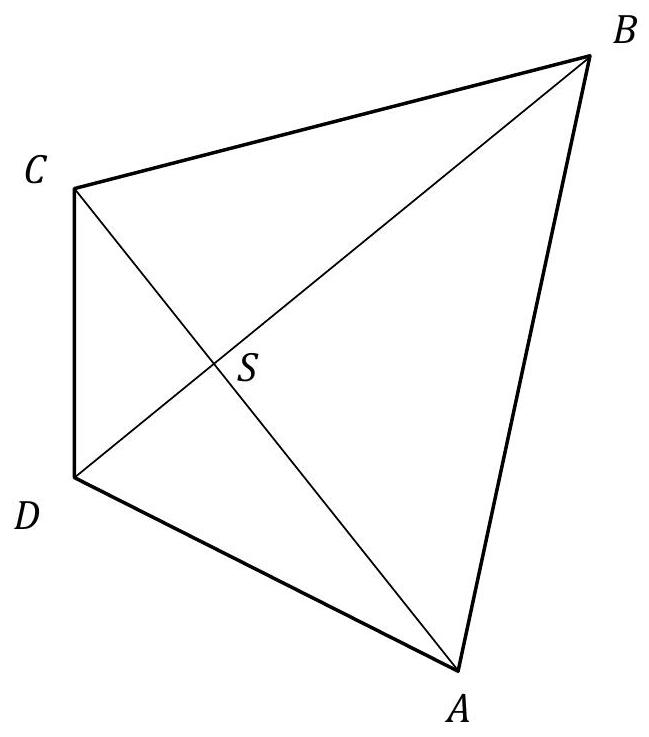
\includegraphics[max width=\textwidth, center]{2025_02_07_d8b842ccd39861fafa8ag-08}

\section*{Zatem}
(1)

$$
|\Varangle D A S|=|\Varangle C B S| \text { oraz }|\Varangle A D S|=|\Varangle B C S| .
$$

Kąty $A S B$ oraz $D S C$ są wierzchołkowe, więc $|\Varangle A S B|=|\Varangle D S C|$. Stąd iz założenia $\frac{|A S|}{|D S|}=\frac{|B S|}{|C S|}$ wnioskujemy, że trójkąty $A S B$ i $D S C$ są podobne na mocy cechy bkb. Zatem


\begin{equation*}
|\Varangle S A B|=|\Varangle S D C| \text { oraz }|\Varangle A B S|=|\Varangle D C S| . \tag{2}
\end{equation*}


Ze związków (1) oraz (2) otrzymujemy

$$
\begin{aligned}
|\Varangle D A B|+|\Varangle B C D| & =|\Varangle D A S|+|\Varangle S A B|+|\Varangle B C S|+|\Varangle D C S|= \\
& =|\Varangle C B S|+|\Varangle S D C|+|\Varangle A D S|+|\Varangle A B S|= \\
& =|\Varangle A B S|+|\Varangle C B S|+|\Varangle S D C|+|\Varangle A D S|= \\
& =|\Varangle A B C|+|\Varangle C D A|
\end{aligned}
$$

Stąd i z twierdzenia o okręgu opisanym na czworokącie wnioskujemy, że na czworokącie $A B C D$ można opisać okrąg.\\
To należało wykazać.

Zadanie 8. (0-3)

\begin{center}
\begin{tabular}{|l|l|}
\hline
\multicolumn{2}{|c|}{Wymagania egzaminacyjne 2024} \\
\hline
\multicolumn{1}{|c|}{Wymaganie ogólne} & \multicolumn{1}{|c|}{Wymaganie szczegółowe} \\
\hline
IV. Użycie i tworzenie strategii. & Zdający: \\
 & 10.1R) wykorzystuje wzory na liczbe \\
 & permutacji, kombinacji, wariacji i wariacji \\
 & z powtórzeniami do zliczania obiektów \\
 & w sytuacjach kombinatorycznych. \\
\hline
\end{tabular}
\end{center}

\section*{Zasady oceniania}
3 pkt - zastosowanie poprawnej metody i poprawny wynik: 11040.\\
2 pkt - zapisanie $L_{1}:\binom{5}{3} \cdot\binom{5}{2} \cdot 5$ ! oraz zapisanie liczby zbiorów czteroelementowych złożonych z trzech cyfr nieparzystych i jednej cyfry parzystej różnej od zera: $\binom{5}{3} \cdot\binom{4}{1}$ ALBO

\begin{itemize}
  \item zapisanie $L_{2}:\binom{5}{3} \cdot\binom{4}{1} \cdot 4$ ! oraz zapisanie liczby zbiorów pięcioelementowych złożonych z trzech cyfr nieparzystych i dwóch cyfr parzystych: $\binom{5}{3} \cdot\binom{5}{2}$, ALBO
  \item zapisanie $P: 4 \cdot\binom{4}{1} \cdot\binom{5}{3} \cdot 4$ ! oraz zapisanie liczby ciągów pięciowyrazowych w jednym z przypadków, w których pierwszy wyraz jest cyfrą nieparzystą, np. liczba ciągów postaci ( $n, p, n, p, n$ ) jest równa $5 \cdot 5 \cdot 4 \cdot 4 \cdot 3$,\\
ALBO
  \item zapisanie $N: 5 \cdot\binom{5}{2} \cdot\binom{4}{2} \cdot 4$ ! oraz zapisanie liczby ciągów pięciowyrazowych w jednym z przypadków, w których pierwszy wyraz jest cyfrą parzystą różną od zera, np. liczba ciągów postaci ( $p, n, n, p, n$ ) jest równa $4 \cdot 5 \cdot 4 \cdot 4 \cdot 3$, ALBO
  \item zapisanie $Z^{+}: 4 \cdot 4 \cdot 4 \cdot 5 \cdot 4 \cdot 3$ oraz zapisanie liczby ciągów pięciowyrazowych $w$ jednym z przypadków, w których żaden wyraz nie jest równy zero, np. liczba ciągów postaci ( $n, n, n, p, p$ ), gdzie $p \in\{2,4,6,8\}$, jest równa $5 \cdot 4 \cdot 3 \cdot 4 \cdot 3$, ALBO
  \item zapisanie $Z^{-}: 10 \cdot 4 \cdot 3 \cdot 5 \cdot 4 \cdot 3$ oraz zapisanie liczby ciągów pięciowyrazowych w jednym z przypadków, w których jeden z wyrazów jest równy zero, np. liczba ciągów postaci ( $p, n, n, n, 0$ ), gdzie $p \in\{2,4,6,8\}$, jest równa $4 \cdot 5 \cdot 4 \cdot 3 \cdot 1$.\\
1 pkt-zapisanie $L_{1}$ (lub $L_{2}$ ), np. $L_{1}=\binom{5}{3} \cdot\binom{5}{2} \cdot 5!, L_{2}=\binom{5}{3} \cdot\binom{4}{1} \cdot 4$ !\\
ALBO
  \item zapisanie $P$ (lub $N$ ), np. $P=4 \cdot\binom{4}{1} \cdot\binom{5}{3} \cdot 4!, N=5 \cdot\binom{5}{2} \cdot\binom{4}{2} \cdot 4$ !, ALBO
  \item zapisanie $Z^{+}$(lub $Z^{-}$), np. $Z^{+}=4 \cdot 4 \cdot 4 \cdot 5 \cdot 4 \cdot 3=3840$, $Z^{-}=10 \cdot 4 \cdot 3 \cdot 5 \cdot 4 \cdot 3=7200$, ALBO
  \item zapisanie liczby zbiorów pięcioelementowych złożonych z trzech cyfr nieparzystych i dwóch cyfr parzystych: $\binom{5}{3} \cdot\binom{5}{2}$ oraz zapisanie liczby zbiorów czteroelementowych złożonych z trzech cyfr nieparzystych i jednej cyfry parzystej różnej od zera: $\binom{5}{3} \cdot\binom{4}{1}$,
\end{itemize}

\section*{ALBO}
\begin{itemize}
  \item zapisanie liczby ciągów pięciowyrazowych w jednym z przypadków, w których pierwszy wyraz jest cyfrą nieparzystą ( $n$. liczba ciągów postaci ( $n, p, n, p, n$ ) jest równa $5 \cdot 5 \cdot 4 \cdot 4 \cdot 3$ ) oraz zapisanie liczby ciągów pięciowyrazowych w jednym z przypadków, w których pierwszy wyraz jest cyfrą parzystą różną od zera (np. liczba ciągów postaci ( $p, n, n, p, n$ ) jest równa $4 \cdot 5 \cdot 4 \cdot 4 \cdot 3$ ).\\
0 pkt - rozwiązanie, w którym zastosowano niepoprawną metodę, albo brak rozwiązania.
\end{itemize}

\section*{Uwaga:}
Jeżeli zdający rozpatruje liczby inne niż pięciocyfrowe, to otrzymuje $\mathbf{0}$ punktów.

\section*{Przykładowe pełne rozwiązania}
\section*{Sposób I}
\section*{Niech $L_{1}$ będzie liczbą wszystkich ciągów pięcioelementowych, których:}
\begin{itemize}
  \item wyrazy są cyframi, parami różnymi
  \item trzy wyrazy są liczbami nieparzystymi, a dwa są liczbami parzystymi.
\end{itemize}

Aby wygenerować taki ciąg należy wybrać trzy cyfry spośród pięciu nieparzystych, dwie cyfry spośród dwóch parzystych i wybrane pięć cyfr ustawić w ciąg. Zatem

$$
L_{1}=\binom{5}{3} \cdot\binom{5}{2} \cdot 5!
$$

Niech $L_{2}$ będzie liczbą wszystkich ciągów pięcioelementowych, których:

\begin{itemize}
  \item wyrazy są cyframi, parami różnymi
  \item pierwszy wyraz jest zerem, a wśród pozostałych wyrazów są trzy cyfry nieparzyste i jedna cyfra parzysta.
\end{itemize}

Aby wygenerować taki ciąg należy wybrać trzy cyfry spośród pięciu nieparzystych oraz jedną cyfrę spośród cyfr: $2,4,6,8$, i wybrane cztery cyfry ustawić w ciąg. Następnie na początku ciągu ustawić cyfrę 0 . Zatem

$$
L_{2}=\binom{5}{3} \cdot\binom{4}{1} \cdot 4!
$$

Wszystkich liczb naturalnych pięciocyfrowych, o różnych cyfrach, w których dokładnie trzy cyfry są nieparzyste, a pozostałe są parzyste, jest

$$
L_{1}-L_{2}=\binom{5}{3} \cdot\binom{5}{2} \cdot 5!-\binom{5}{3} \cdot\binom{4}{1} \cdot 4!=10 \cdot 10 \cdot 120-10 \cdot 4 \cdot 24=11040
$$

\section*{Sposób II}
Niech $P$ będzie liczbą wszystkich ciągów pięcioelementowych, których:

\begin{itemize}
  \item wyrazy są cyframi, parami różnymi
  \item pierwszy wyraz jest cyfrą parzystą różną od zera, a wśród pozostałych wyrazów są trzy cyfry nieparzyste i jedna cyfra parzysta.
\end{itemize}

Pierwszy wyraz takiego ciągu można ustalić na cztery sposoby (wybieramy jedną cyfrę parzystą spośród $2,4,6,8$ ). Pozostałe wyrazy można ustalić poprzez wybór jednej cyfry parzystej spośród czterech, trzech cyfr nieparzystych spośród pięciu, a następnie ustawienie wybranych czterech cyff na ostatnich czterech pozycjach w ciągu. Zatem

$$
P=4 \cdot\binom{4}{1} \cdot\binom{5}{3} \cdot 4!
$$

Niech $N$ będzie liczbą wszystkich ciągów pięcioelementowych, których:

\begin{itemize}
  \item wyrazy są cyframi, parami różnymi
  \item pierwszy wyraz jest cyfrą nieparzystą, a wśród pozostałych wyrazów są dwie cyfry nieparzyste i dwie cyfry parzyste.
\end{itemize}

Pierwszy wyraz takiego ciągu można ustalić na pięć sposobów (wybieramy jedną cyfrę nieparzystą spośród pięciu). Pozostałe wyrazy można ustalić poprzez wybór dwóch cyfr parzystych spośród pięciu, dwóch cyfr nieparzystych spośród czterech, a następnie ustawienie wybranych czterech cyfr na ostatnich czterech pozycjach w ciągu. Zatem

$$
N=5 \cdot\binom{5}{2} \cdot\binom{4}{2} \cdot 4!
$$

Wszystkich liczb naturalnych pięciocyfrowych, o różnych cyfrach, w których dokładnie trzy cyfry są nieparzyste, a pozostałe są parzyste, jest

$$
P+N=4 \cdot\binom{4}{1} \cdot\binom{5}{3} \cdot 4!+5 \cdot\binom{5}{2} \cdot\binom{4}{2} \cdot 4!=4 \cdot 4 \cdot 10 \cdot 24+5 \cdot 10 \cdot 6 \cdot 24=11040
$$

\section*{Sposób III}
Rozważmy dwa przypadki:

\begin{enumerate}
  \item Gdy w zapisie liczby występuje cyfra zero. Cyfrę tę możemy wstawić na jedno z 4 miejsc. Miejsce dla drugiej, różnej od zera cyfry parzystej możemy wybrać na 4 sposoby, a na wybranym miejscu możemy wstawić jedną z pozostałych 4 cyfr parzystych. Na pierwsze z pozostałych trzech wolnych miejsc możemy wstawić jedną z 5 cyfr nieparzystych, na drugie z pozostałych dwóch wolnych miejsc możemy wstawić jedną z pozostałych 4 cyfr nieparzystych, a na ostatnim wolnym miejscu - jedną z pozostałych 3 cyfr nieparzystych. Zatem liczba $Z^{+}$wszystkich rozpatrywanych liczb w tym przypadku jest równa
\end{enumerate}

$$
Z^{+}=4 \cdot 4 \cdot 4 \cdot 5 \cdot 4 \cdot 3=3840
$$

\begin{enumerate}
  \setcounter{enumi}{1}
  \item Gdy w zapisie liczby nie występuje cyfra zero. Dwa miejsca dla cyfr parzystych możemy wybrać na $\binom{5}{2}=10$ sposobów. Na pierwsze z wybranych dwóch miejsc możemy wstawić jedną z 4 cyfr parzystych, a na drugie - jedną z 3. Na pierwsze z pozostałych trzech wolnych miejsc możemy wstawić jedną z 5 cyfr nieparzystych, na drugie z pozostałych dwóch wolnych miejsc możemy wstawić jedną z pozostałych 4 cyfr nieparzystych, a na ostatnim wolnym miejscu - jedną z pozostałych 3 cyfr nieparzystych. Zatem liczba $Z^{-}$wszystkich rozpatrywanych liczb w tym przypadku jest równa
\end{enumerate}

$$
Z^{-}=10 \cdot 4 \cdot 3 \cdot 5 \cdot 4 \cdot 3=7200
$$

Stąd wszystkich rozważanych liczb jest $Z^{+}+Z^{-}=3840+7200=11040$.

\section*{Zadanie 9. (0-3)}
\begin{center}
\begin{tabular}{|l|l|}
\hline
\multicolumn{2}{|c|}{Wymagania egzaminacyjne 2024} \\
\hline
\multicolumn{1}{|c|}{Wymaganie ogólne} & \multicolumn{1}{c|}{Wymagania szczegółowe} \\
\hline
II. Wykorzystanie i interpretowanie & Zdający: \\
reprezentacji. & 11.2R) oblicza pochodne funkcji \\
 & wymiernych; \\
 & 11.3R) korzysta z geometrycznej \\
 & interpretacji pochodnej. \\
\hline
\end{tabular}
\end{center}

\section*{Zasady oceniania}
3 pkt - zastosowanie poprawnej metody i poprawny wynik: $a=\frac{7}{2}$ oraz $b=-5$.\\
2 pkt - obliczenie współczynnika kierunkowego stycznej do wykresu funkcji $f$ w punkcie $P$ :

$$
a=f^{\prime}(2)=\frac{7}{2} .
$$

1 pkt - wyznaczenie pochodnej funkcji $f$, np. $f^{\prime}(x)=\frac{\left(3 x^{2}-3\right) \cdot x-\left(x^{3}-3 x+2\right) \cdot 1}{x^{2}}$,

$$
f^{\prime}(x)=2 x+2 \cdot\left(-\frac{1}{x^{2}}\right)
$$

0 pkt - rozwiązanie, w którym zastosowano niepoprawną metodę, albo brak rozwiązania.

\section*{Uwaga:}
Jeżeli zdający błędnie zastosuje wzór na pochodną ilorazu funkcji lub błędnie obliczy pochodną funkcji $y=x^{3}-3 x+2$, lub $y=x$, to może otrzymać 1 punkt za całe rozwiązanie, o ile nie popełni błędu w obliczaniu współczynnika $a$ oraz $b$.

\section*{Przykładowe pełne rozwiązanie}
Wyznaczamy pochodną funkcji $f$ :

$$
\begin{gathered}
f^{\prime}(x)=\frac{\left(3 x^{2}-3\right) \cdot x-\left(x^{3}-3 x+2\right) \cdot 1}{x^{2}} \\
f^{\prime}(x)=\frac{2 x^{3}-2}{x^{2}}
\end{gathered}
$$

Obliczamy współczynnik kierunkowy a w równaniu stycznej:

$$
a=f^{\prime}(2)=\frac{7}{2}
$$

Obliczamy współczynnik b w równaniu stycznej:

$$
\begin{gathered}
f(2)=\frac{7}{2} \cdot 2+b \\
2=7+b \\
b=-5
\end{gathered}
$$

Współczynniki w równaniu stycznej są równe: $a=\frac{7}{2}$ oraz $b=-5$.

Zadanie 10. (0-3)

\begin{center}
\begin{tabular}{|l|l|}
\hline
\multicolumn{2}{|c|}{Wymagania egzaminacyjne 2024} \\
\hline
\multicolumn{1}{|c|}{Wymaganie ogólne} & \multicolumn{1}{|c|}{Wymagania szczegółowe} \\
\hline
III. Modelowanie matematyczne. & Zdający: \\
 & 10.1R) wykorzystuje wzory na liczbę [...] \\
 & kombinacji [...]. \\
 & 10.2) oblicza prawdopodobieństwa [...]. \\
\hline
\end{tabular}
\end{center}

\section*{Zasady oceniania}
3 pkt - zastosowanie poprawnej metody i poprawny wynik: $P(A)=\frac{28}{8^{6}}=\frac{7}{65536}$.\\
2 pkt - zapisanie liczby $|\Omega|$ wszystkich zdarzeń elementarnych oraz zapisanie liczby $|A|$ wszystkich zdarzeń elementarnych sprzyjających zdarzeniu $A, \mathrm{np} .|\Omega|=8^{6}$ oraz $|A|=\binom{8}{6}$ ALBO

\begin{itemize}
  \item zapisanie liczby $|\Omega|$ wszystkich zdarzeń elementarnych oraz wypisanie wszystkich zdarzeń elementarnych sprzyjających zdarzeniu $A$ i niewypisanie żadnego zdarzenia niewłaściwego, np. $|\Omega|=8^{6}$ oraz
\end{itemize}

$$
\begin{aligned}
A= & \{876543,876542,876541,876532,876531,876521,876432,876431, \\
& 876421,876321,875432,875431,875421,875321,874321,865432, \\
& 865431,865421,865321,864321,854321,765432,765431,765421, \\
& 765321,764321,754321,654321\} .
\end{aligned}
$$

1 pkt - zapisanie liczby $|\Omega|$ wszystkich zdarzeń elementarnych: np. $|\Omega|=8^{6}$ ALBO

\begin{itemize}
  \item zapisanie liczby $|A|$ wszystkich zdarzeń elementarnych sprzyjających zdarzeniu $A$ : np. $|A|=\binom{8}{6}$,\\
ALBO
  \item wypisanie wszystkich zdarzeń elementarnych sprzyjających zdarzeniu $A$ i niewypisanie żadnego zdarzenia niewłaściwego:\\
654321, 765432, 765321, 876543, 875432, 865432, 864321, 854321, 765431, 764321, 876542, 875431, 865431, 765421, 754321, 876541, 875421, 865421, 876532, 875321, 865321, 876531, 874321, 876521, 876432, 876431, 876421, 876321.
\end{itemize}

0 pkt - rozwiązanie, w którym zastosowano niepoprawną metodę, albo brak rozwiązania.

\section*{Przykładowe pełne rozwiązanie}
Zdarzeniem elementarnym jest sześciowyrazowy ciąg o wyrazach ze zbioru\\
$\{1,2,3,4,5,6,7,8\}$, więc liczba $|\Omega|$ wszystkich zdarzeń elementarnych jest równa $|\Omega|=8^{6}$.\\
Niech $A$ oznacza zdarzenie polegające na tym, że wylosowano liczbę, której druga cyfra (licząc od lewej strony) jest mniejsza od pierwszej, a każda następna cyfra tej liczby jest mniejsza od poprzedniej. Wtedy zdarzeniem elementarnym sprzyjającym zdarzeniu $A$ jest sześciowyrazowy ciąg malejący. Liczba wszystkich takich ciągów jest równa $\binom{8}{6}$, więc $|A|=\binom{8}{6}$.\\
Obliczamy prawdopodobieństwo zdarzenia $A$ :

$$
P(A)=\frac{|A|}{|\Omega|}=\frac{\binom{8}{6}}{8^{6}}=\frac{28}{262144}=\frac{7}{65536}
$$

Zadanie 11. (0-4)

\begin{center}
\begin{tabular}{|l|l|}
\hline
\multicolumn{2}{|c|}{Wymagania egzaminacyjne 2024} \\
\hline
\multicolumn{1}{|c|}{Wymaganie ogólne} & \multicolumn{1}{|c|}{Wymagania szczegółowe} \\
\hline
III. Modelowanie matematyczne. & Zdający: \\
 & \begin{tabular}{l}
5.3) stosuje wzór na $n$-ty wyraz [...] ciągu \\
arytmetycznego; \\
 \\
 \\
 \\
 \\
 \\
 \\
 \\
 \\
5.4) stosuje wzór na $n$-ty wyraz [...] ciągu \\
geometrycznego. \\
\hline
\end{tabular} \\
\hline
\end{tabular}
\end{center}

\section*{Zasady oceniania (dla sposobu I ill)}
4 pkt - zastosowanie poprawnej metody i poprawny wynik: $x=5, y=20, z=80$.\\
3 pkt - zapisanie równania z jedną niewiadomą $r$, np. $(35-r)^{2}=(35-2 r) \cdot(35+3 r)$ ALBO

\begin{itemize}
  \item poprawne wyznaczenie $r$ w zależności od $x$ z równania $(x+r)^{2}=x(x+5 r)$ : $r=3 x$.\\
2 pkt-zapisanie $x, y$ oraz $z$ w zależności od $r: x=35-2 r, y=35-r, z=35+3 r$ ALBO
  \item zapisanie układu równań\\
$x+x+r+x+5 r=105$ i $(x+r)^{2}=x(x+5 r)$ lub\\
$x+x+r+x+5 r=105$ i $x+x \cdot \frac{x+5 r}{x+r}+x \cdot\left(\frac{x+5 r}{x+r}\right)^{2}=105$\\
1 pkt - zapisanie równania $x+x+r+x+5 r=105$\\
ALBO
  \item zapisanie równania $(x+r)^{2}=x(x+5 r)$,
\end{itemize}

ALBO

\begin{itemize}
  \item zapisanie równania $x+x \cdot \frac{x+5 r}{x+r}+x \cdot\left(\frac{x+5 r}{x+r}\right)^{2}=105$.
\end{itemize}

0 pkt - rozwiązanie, w którym zastosowano niepoprawną metodę, albo brak rozwiązania.

\section*{Zasady oceniania (dla sposobu III)}
4 pkt - zastosowanie poprawnej metody i poprawny wynik: $x=5, y=20, z=80$.\\
3 pkt - zapisanie równania $z$ jedną niewiadomą $y$, np. $y^{2}=(2 y-35) \cdot(140-3 y)$.\\
2 pkt-zapisanie $x$ oraz $z$ w zależności od $y: x=2 y-35, z=140-3 y$.\\
1 pkt - zapisanie równania $4 \cdot(y-x)=z-y$ lub $y^{2}=x z$, lub $5(y-x)=z-x$.\\
0 pkt - rozwiązanie, w którym zastosowano niepoprawną metodę, albo brak rozwiązania.

\section*{Zasady oceniania (dla sposobu IV)}
4 pkt - zastosowanie poprawnej metody i poprawny wynik: $x=5, y=20, z=80$.\\
3 pkt -zapisanie równania $x+x \cdot q+x \cdot q^{2}=105$ oraz obliczenie $q: q=4$\\
ALBO

\begin{itemize}
  \item zapisanie równania $x+x \cdot q+x \cdot q^{2}=105$ oraz zapisanie, że ciąg $(x, y, z)$ jest rosnący, więc $x \neq 0$, oraz zapisanie równania $q^{2}-5 q+4=0$.\\
2 pkt - zapisanie równania $4 \cdot(x \cdot q-x)=x \cdot q^{2}-x \cdot q$ oraz zapisanie, że ciąg $(x, y, z)$ jest rosnący, więc $x \neq 0$ i $q \neq 1$, oraz obliczenie $q: q=4$
\end{itemize}

\section*{ALBO}
\begin{itemize}
  \item zapisanie równań $4 \cdot(x \cdot q-x)=x \cdot q^{2}-x \cdot q$ oraz
\end{itemize}

$$
x+x \cdot q+x \cdot q^{2}=105
$$

1 pkt - zapisanie równania $4 \cdot(x \cdot q-x)=x \cdot q^{2}-x \cdot q$ lub $x+x \cdot q+x \cdot q^{2}=105$. 0 pkt - rozwiązanie, w którym zastosowano niepoprawną metodę, albo brak rozwiązania.

\section*{Uwagi:}
\begin{enumerate}
  \item Jeżeli zdający dzieli obie strony otrzymanego równania przez wyrażenie zawierające niewiadomą i nie umieszcza zapisu, że to wyrażenie jest różne od zera, oraz konsekwentnie rozwiąże zadanie do końca, to może otrzymać co najwyżej 3 punkty za całe rozwiązanie.
  \item Jeżeli zdający popełni błąd, który nie jest rachunkowy, np. $\frac{a_{1}+a_{1}+5 r}{2} \cdot 6=105$, $y-x=4 \cdot(z-y)$ i rozwiąże zadanie do końca, to może otrzymać co najwyżej 2 punkty za całe rozwiązanie (za spełnienie kryterium z kategorii za 1 pkt oraz za obliczenie $x, y$ oraz $z$ ).
\end{enumerate}

\section*{Przykładowe pełne rozwiązania}
Sposób I\\
Niech $r$ będzie różnicą ciągu arytmetycznego $\left(a_{n}\right)$. Wtedy $y=x+r$ oraz $z=x+5 r$.\\
Ponieważ $x+y+z=105$, więc

$$
\begin{gathered}
x+(x+r)+(x+5 r)=105 \\
x+2 r=35 \\
x=35-2 r
\end{gathered}
$$

Zatem $y=35-2 r+r=35-r$ oraz $z=35-2 r+5 r=35+3 r$.\\
$Z$ własności ciągu geometrycznego otrzymujemy

$$
\begin{gathered}
y^{2}=x \cdot z \\
(35-r)^{2}=(35-2 r) \cdot(35+3 r) \\
35^{2}-70 r+r^{2}=35^{2}+35 r-6 r^{2} \\
7 r^{2}-105 r=0 \\
r=0 \vee r=15
\end{gathered}
$$

Dla $r=0$ otrzymujemy $x=y=z$, więc warunki zadania nie są spełnione.\\
Dla $r=15$ otrzymujemy $x=5, y=20, z=80$. Ciąg ( $5,20,80$ ) jest geometryczny i rosnący. Suma wyrazów tego ciągu jest równa 105 . Ponadto wyrazy tego ciągu są odpowiednio - pierwszym, drugim i szóstym wyrazem ciągu arytmetycznego określonego wzorem $a_{n}=5+15 n$, gdzie $n \in \mathbb{N}_{+}$.\\
Zatem ostatecznie $x=5, y=20, z=80$.

\section*{Sposób II}
Niech $r$ będzie różnicą ciągu arytmetycznego $\left(a_{n}\right)$. Wtedy $y=x+r$ oraz $z=x+5 r$. Ponieważ $x+y+z=105$, więc

$$
x+(x+r)+(x+5 r)=105
$$

Z własności ciągu geometrycznego otrzymujemy

$$
y^{2}=x \cdot z
$$

Ponieważ $y=x+r$ oraz $z=x+5 r$, więc

$$
(x+r)^{2}=x \cdot(x+5 r)
$$

Zatem otrzymujemy układ dwóch równań z niewiadomymi $x$ oraz $r$ :

$$
\left\{\begin{array}{l}
x+x+r+x+5 r=105 \\
(x+r)^{2}=x(x+5 r)
\end{array}\right.
$$

Ze związku $(x+r)^{2}=x \cdot(x+5 r)$ otrzymujemy kolejno:

$$
\begin{gathered}
x^{2}+2 x r+r^{2}=x^{2}+5 x r \\
r^{2}-3 r x=0 \\
r=0 \vee r=3 x
\end{gathered}
$$

Dla $r=0$ otrzymujemy $x=y=z$, więc warunki zadania nie są spełnione.\\
Dla $r=3 x$ otrzymujemy

$$
\left\{\begin{array}{l}
3 x+6 r=105 \\
r=3 x
\end{array}\right.
$$

Rozwiązaniem tego układu równań jest para liczb $\left\{\begin{array}{l}x=5 \\ r=15\end{array}\right.$\\
Stąd $y=x+r=5+15=20$ oraz $z=x+5 r=5+75=80$.\\
Ciąg ( $5,20,80$ ) jest geometryczny i rosnący. Suma wyrazów tego ciągu jest równa 105.\\
Ponadto wyrazy tego ciągu są - odpowiednio - pierwszym, drugim i szóstym wyrazem ciągu arytmetycznego określonego wzorem $a_{n}=5+15 n$, gdzie $n \in \mathbb{N}_{+}$.\\
Zatem ostatecznie $x=5, y=20, z=80$.

\section*{Sposób III}
Z warunków zadania oraz z własności ciągów geometrycznego i arytmetycznego otrzymujemy zależności między $x, y$ oraz $z$ :

$$
\begin{gathered}
x+y+z=105 \\
y^{2}=x z \\
4 \cdot(y-x)=z-y
\end{gathered}
$$

Rozwiązujemy układ tych trzech równań:

$$
\left\{\begin{array}{l}
z=105-x-y \\
y^{2}=x \cdot(105-x-y) \\
4 \cdot(y-x)=105-x-y-y
\end{array}\right.
$$

$$
\begin{aligned}
& \left\{\begin{array}{l}
z=105-x-y \\
y^{2}=x \cdot(105-x-y) \\
x=2 y-35
\end{array}\right. \\
& \left\{\begin{array}{l}
z=140-3 y \\
y^{2}=(2 y-35) \cdot(140-3 y) \\
x=2 y-35
\end{array}\right. \\
& \left\{\begin{array}{l}
z=140-3 y \\
7 y^{2}-385 y+4900=0 \\
x=2 y-35
\end{array}\right. \\
& \left\{\begin{array} { l } 
{ z = 8 0 } \\
{ y = 2 0 } \\
{ x = 5 }
\end{array} \vee \left\{\begin{array}{l}
z=35 \\
y=35 \\
x=35
\end{array}\right.\right.
\end{aligned}
$$

Dla $x=y=z=35$ warunki zadania nie są spełnione.\\
Ciąg $(5,20,80)$ jest geometryczny i rosnący. Suma wyrazów tego ciągu jest równa 105.\\
Ponadto wyrazy tego ciągu są - odpowiednio - pierwszym, drugim i szóstym wyrazem ciągu arytmetycznego określonego wzorem $a_{n}=5+15 n$, gdzie $n \in \mathbb{N}_{+}$.\\
Zatem $x=5, y=20, z=80$.

\section*{Sposób IV}
Niech $q$ będzie ilorazem ciągu geometrycznego $(x, y, z)$. Wtedy $y=x \cdot q$ oraz $z=x \cdot q^{2}$. Z warunków zadania oraz własności ciągu arytmetycznego otrzymujemy

$$
\begin{gathered}
4 \cdot(y-x)=z-y \\
4 \cdot(x \cdot q-x)=x \cdot q^{2}-x \cdot q
\end{gathered}
$$

Ponieważ ciąg $(x, y, z)$ jest rosnący, więc $x \neq 0$ i $q \neq 1$. Zatem

$$
\begin{aligned}
4 \cdot(x \cdot q-x) & =x \cdot q^{2}-x \cdot q \\
4 \cdot x \cdot(q-1) & =x \cdot q \cdot(q-1) \\
4 & =q
\end{aligned}
$$

Z warunków zadania $x+y+z=105$, więc $x+x \cdot q+x \cdot q^{2}=105$ i dalej $x+x \cdot 4+x \cdot 4^{2}=105$. Stąd otrzymujemy $x=5$. Wówczas $y=5 \cdot 4=20$ oraz $z=5 \cdot 4^{2}=80$.\\
Ciąg ( $5,20,80$ ) jest geometryczny i rosnący. Suma wyrazów tego ciągu jest równa 105. Ponadto wyrazy tego ciągu są - odpowiednio - pierwszym, drugim i szóstym wyrazem ciągu arytmetycznego określonego wzorem $a_{n}=5+15 n$, gdzie $n \in \mathbb{N}_{+}$.\\
Zatem $x=5, y=20, z=80$.

Zadanie 12. (0-4)

\begin{center}
\begin{tabular}{|l|l|}
\hline
\multicolumn{2}{|c|}{Wymagania egzaminacyjne 2024} \\
\hline
\multicolumn{1}{|c|}{Wymaganie ogólne} & \multicolumn{1}{c|}{Wymagania szczegółowe} \\
\hline
IV. Użycie i tworzenie strategii. & Zdający: \\
 & 6.5R) stosuje wzory na sinus i cosinus sumy \\
 & i różnicy kątów, sumę i różnicę sinusów \\
 & i cosinusów kąów; \\
 & $6.6 \mathrm{R})$ rozwiązuje równania \\
 & trygonometryczne typu $\sin 2 x=\frac{1}{2}$, \\
 & $\sin 2 x+\cos x=1, \sin x+\cos x=1$. \\
\hline
\end{tabular}
\end{center}

\section*{Zasady oceniania}
4 pkt - poprawna metoda rozwiązania równania i poprawne wyniki: $\frac{\pi}{4}, \frac{7 \pi}{6}, \frac{5 \pi}{4}$ oraz $\frac{11 \pi}{6}$. 3 pkt - rozwiązanie równań $\sin x=\cos x$ oraz $\sin x=-\frac{1}{2} \mathrm{w}$ zbiorze $\mathbb{R}: \frac{\pi}{4}+k \cdot \pi$ oraz $\frac{7 \pi}{6}+2 k \cdot \pi$ i $\frac{11 \pi}{6}+2 k \cdot \pi$, gdzie $k \in \mathbb{Z}$\\
ALBO

\begin{itemize}
  \item rozwiązanie równania $\sin x=\cos x$ (lub równania $\sin x=-\frac{1}{2}$ ) w zbiorze $\langle 0,2 \pi\rangle$ : $\frac{\pi}{4}$ oraz $\frac{5 \pi}{4}$ (lub: $\frac{7 \pi}{6}$ oraz $\frac{11 \pi}{6}$ ).\\
2 pkt - przekształcenie równoważne równania $\sin (2 x)+\cos (2 x)=1+\sin x-\cos x$ do postaci $(\sin x-\cos x)(2 \sin x+1)=0$.\\
1 pkt - zastosowanie wzorów na sinus oraz cosinus podwojonego kąta.\\
0 pkt - rozwiązanie, w którym zastosowano niepoprawną metodę, albo brak rozwiązania.
\end{itemize}

\section*{Uwaga:}
Jeżeli zdający podczas przekształcania równania $\sin (2 x)+\cos (2 x)=1+\sin x-\cos x$ podzieli obie strony równania przez $(\cos x-\sin x)$ bez stosownych założeń i konsekwentnie do popełnionego błędu rozwiąże zadanie do końca, to otrzymuje 2 punkty za całe rozwiązanie.

\section*{Przykładowe pełne rozwiązanie}
Przekształcamy równanie $\sin (2 x)+\cos (2 x)=1+\sin x-\cos x$ równoważnie, korzystając ze wzorów na sinus oraz cosinus podwojonego kąta, i otrzymujemy:

$$
\begin{gathered}
\sin (2 x)+\cos (2 x)=1+\sin x-\cos x \\
2 \sin x \cdot \cos x+\cos ^{2} x-\sin ^{2} x=1+\sin x-\cos x \\
\cos ^{2} x-\sin ^{2} x=1-2 \sin x \cdot \cos x+\sin x-\cos x \\
0=(\sin x-\cos x)^{2}+\sin x-\cos x+\sin ^{2} x-\cos ^{2} x \\
0=(\sin x-\cos x)^{2}+(\sin x-\cos x)+(\sin x-\cos x)(\sin x+\cos x)
\end{gathered}
$$

$$
\begin{gathered}
0=(\sin x-\cos x)(\sin x-\cos x+1+\sin x+\cos x) \\
0=(\sin x-\cos x)(2 \sin x+1) \\
\sin x=\cos x \text { lub } \sin x=-\frac{1}{2}
\end{gathered}
$$

Rozwiązujemy równanie $\sin x=\cos x$ w zbiorze $\langle 0,2 \pi\rangle$.\\
Zauważmy, że gdyby $\cos x=0$, to wtedy $\sin x=\cos x=0$, więc po podstawieniu tych wartości sinusa i cosinusa do tożsamości $\sin ^{2} x+\cos ^{2} x=1$ otrzymalibyśmy $0+0=1$. Zatem $\cos x \neq 0$.\\
Dzielimy obie strony równania $\sin x=\cos x$ przez $\cos x$ i otrzymujemy $\operatorname{tg} x=1$.\\
Równanie to ma w zbiorze $\langle 0,2 \pi\rangle$ dwa rozwiązania: $\frac{\pi}{4}$ oraz $\frac{5 \pi}{4}$.\\
Równanie $\sin x=-\frac{1}{2}$ ma w zbiorze $\langle 0,2 \pi\rangle$ dwa rozwiązania: $\frac{7 \pi}{6}$ oraz $\frac{11 \pi}{6}$.\\
Ostatecznie równanie $\sin (2 x)+\cos (2 x)=1+\sin x-\cos x$ ma w zbiorze $\langle 0,2 \pi\rangle$ cztery rozwiązania: $\frac{\pi}{4}, \frac{7 \pi}{6}, \frac{5 \pi}{4}$ oraz $\frac{11 \pi}{6}$.

Zadanie 13. (0-4)

\begin{center}
\begin{tabular}{|l|l|}
\hline
\multicolumn{2}{|c|}{Wymagania egzaminacyjne 2024} \\
\hline
\multicolumn{1}{|c|}{Wymaganie ogólne} & \multicolumn{1}{c|}{Wymaganie szczegółowe} \\
\hline
IV. Użycie i tworzenie strategii. & \begin{tabular}{l}
Zdający: \\
 \\
 \\
 \\
 \\
 \\
 \\
 \\
 \\
 \\
 \\
7.4R) znajduje związki miarowe w figurach z zastosowaniem twierdzenia \\
pinusów i twierdzenia cosinusów. \\
\end{tabular} \\
\hline
\end{tabular}
\end{center}

\section*{Zasady oceniania}
4 pkt - zastosowanie poprawnej metody i poprawny wynik: $15 \sqrt{3}+8$ (lub

$$
\sqrt{739+240 \sqrt{3}}) .
$$

3 pkt - zapisanie równania z jedną niewiadomą (długością boku $A C$ ), np.

$$
\begin{aligned}
& 17^{2}=|A C|^{2}+30^{2}-2 \cdot 30 \cdot|A C| \cdot \frac{\sqrt{3}}{2}, \\
& |A C|^{2}=30^{2}+17^{2}-2 \cdot 30 \cdot 17 \cdot \frac{15-8 \sqrt{3}}{34}, \\
& 30^{2}=|A C|^{2}+17^{2}-2 \cdot|A C| \cdot 17 \cdot \frac{8}{17} \\
& A L B O
\end{aligned}
$$

\begin{itemize}
  \item obliczenie długości odcinków $B D$ oraz $A D:|B D|=15$ oraz $|A D|=15 \sqrt{3}$ (dla sposobu II),\\
ALBO
  \item obliczenie sinusa kąta $A B C: \frac{15 \sqrt{3}+8}{34}$ (dla sposobu III).
\end{itemize}

2 pkt - obliczenie miary kąta $B A C: 30^{\circ}$.\\
1 pkt - zapisanie, że kąt $B S C$ ma miarę $60^{\circ}$\\
ALBO

\begin{itemize}
  \item zapisanie równania, w którym jedyną niewiadomą jest miara kąta $B A C$ (lub miara kąta $A C B)$, np. $\frac{17}{\sin |\Varangle B A C|}=34, \frac{30}{\sin |\Varangle A C B|}=34, \frac{1}{2} \cdot 30 \cdot \sin |\Varangle B A C|=\frac{30 \cdot 17}{4 \cdot 17}$, ALBO
  \item zapisanie układu równań: $|A C|^{2}=30^{2}+17^{2}-2 \cdot 30 \cdot 17 \cdot \cos |\Varangle A B C|$ oraz
\end{itemize}

$$
\frac{|A C|}{\sin |\Varangle A B C|}=34 .
$$

0 pkt - rozwiązanie, w którym zastosowano niepoprawną metodę, albo brak rozwiązania.

\section*{Przykładowe pełne rozwiązania}
Sposób 1\\
Oznaczmy przez $S$ środek okręgu opisanego na trójkącie $A B C$, a przez $R$ - promień tego okręgu. Ponieważ $R=17$ oraz $|B C|=17$, więc trójkąt $B S C$ jest równoboczny. Punkt $A$ leży na dłuższym z łuków $B C$ okręgu opisanego na trójkącie, gdyż gdyby leżał na krótszym, to wtedy odcinek $B C$ byłby najdłuższym bokiem trójkąta $A B C$. Zatem miara kąta wpisanego $B A C$ jest połową miary kąta $B S C$ trójkąta równobocznego, czyli $|\Varangle B A C|=30^{\circ}$. Stosujemy do trójkąta $A B C$ twierdzenie cosinusów i obliczamy długość boku $A C$ :

$$
\begin{gathered}
|B C|^{2}=|A C|^{2}+|A B|^{2}-2 \cdot|A B| \cdot|A C| \cdot \cos |\not \subset B A C| \\
17^{2}=|A C|^{2}+30^{2}-2 \cdot 30 \cdot|A C| \cdot \frac{\sqrt{3}}{2} \\
|A C|^{2}-30 \sqrt{3} \cdot|A C|+611=0 \\
|A C|=15 \sqrt{3}+8 \quad \vee \quad|A C|=15 \sqrt{3}-8
\end{gathered}
$$

Ponieważ $15 \sqrt{3}-8<30$, więc ostatecznie $|A C|=15 \sqrt{3}+8$.

\section*{Sposób II}
Oznaczmy przez $S$ środek okręgu opisanego na trójkącie $A B C$, a przez $R$ - promień tego okręgu.\\
Stosujemy do trójkąta $A B C$ twierdzenie sinusów i otrzymujemy:

$$
\begin{aligned}
& \frac{|B C|}{\sin |\measuredangle B A C|}=2 R \\
& \frac{17}{\sin |\Varangle B A C|}=34
\end{aligned}
$$

Stąd $|\Varangle B A C|=30^{\circ}$ lub $|\Varangle B A C|=150^{\circ}$. Ponieważ bok $B C$ nie jest najdłuższym bokiem trójkąta $A B C$, więc kąt leżący naprzeciw tego boku nie może być rozwarty. Zatem $|\Varangle B A C|=30^{\circ}$.\\
Niech $D$ będzie spodkiem wysokości poprowadzonej w trójkącie $A B C$ z wierzchołka $B$ na bok $A C$ (zobacz rysunek).\\
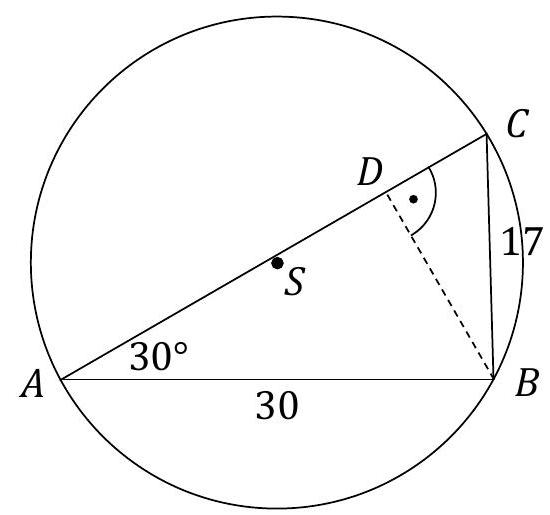
\includegraphics[max width=\textwidth, center]{2025_02_07_d8b842ccd39861fafa8ag-22}

Korzystamy ze związków miarowych dla trójkąta o kątach $30^{\circ}, 60^{\circ}, 90^{\circ}$ i otrzymujemy\\
$|B D|=\frac{1}{2} \cdot|A B|=15$ oraz $|A D|=\frac{\sqrt{3}}{2} \cdot|A B|=15 \sqrt{3}$.\\
Stosujemy do trójkąta $B C D$ twierdzenie Pitagorasa i otrzymujemy

$$
|C D|=\sqrt{|C B|^{2}-|B D|^{2}}=\sqrt{17^{2}-15^{2}}=8
$$

Zatem $|A C|=|A D|+|C D|=15 \sqrt{3}+8$.

\section*{Sposób III}
Oznaczmy przez $S$ środek okręgu opisanego na trójkącie $A B C$, a przez $R$ - promień tego okręgu.\\
Stosujemy do trójkąta $A B C$ twierdzenie sinusów i otrzymujemy:

$$
\begin{aligned}
& \frac{|B C|}{\sin |\Varangle B A C|}=2 R \\
& \frac{17}{\sin |\Varangle B A C|}=34
\end{aligned}
$$

Stąd $|\Varangle B A C|=30^{\circ}$ lub $|\Varangle B A C|=150^{\circ}$. Ponieważ bok $B C$ nie jest najdłuższym bokiem trójkąta $A B C$, więc kąt leżący naprzeciw tego boku nie może być rozwarty. Zatem $|\Varangle B A C|=30^{\circ}$.\\
Ponownie stosujemy do trójkąta $A B C$ twierdzenie sinusów i obliczamy sinus kąta $A C B$ :

$$
\begin{aligned}
& \frac{|A B|}{\sin |\Varangle A C B|}=2 R \\
& \frac{30}{\sin |\Varangle A C B|}=34 \\
& \sin |\Varangle A C B|=\frac{15}{17}
\end{aligned}
$$

Korzystamy z jedynki trygonometrycznej i otrzymujemy

$$
\begin{gathered}
\sin ^{2}|\Varangle A C B|+\cos ^{2}|\Varangle A C B|=1 \\
\left(\frac{15}{17}\right)^{2}+\cos ^{2}|\Varangle A C B|=1 \\
\cos |\Varangle A C B|=\frac{8}{17} \quad \vee \cos |\Varangle A C B|=-\frac{8}{17}
\end{gathered}
$$

Ponieważ $A B$ nie jest najdłuższym bokiem trójkąta, więc kąt $A C B$ nie jest rozwarty i dlatego $\cos |\Varangle A C B|=\frac{8}{17}$.\\
Obliczamy $\sin |\Varangle A B C|$ :

$$
\begin{aligned}
\sin |\Varangle A B C| & =\sin \left(180^{\circ}-|\Varangle B A C|-|\Varangle A C B|\right)=\sin (|\Varangle B A C|+|\Varangle A C B|)= \\
& =\sin |\Varangle B A C| \cdot \cos |\Varangle A C B|+\sin |\Varangle A C B| \cdot \cos |\Varangle B A C|= \\
& =\frac{1}{2} \cdot \frac{8}{17}+\frac{15}{17} \cdot \frac{\sqrt{3}}{2}=\frac{15 \sqrt{3}+8}{34}
\end{aligned}
$$

Stosujemy do trójkąta $A B C$ twierdzenie sinusów i otrzymujemy

$$
\begin{gathered}
\frac{|A C|}{\sin |\Varangle A B C|}=2 R \\
|A C|=2 R \cdot \sin |\Varangle A B C|
\end{gathered}
$$

$$
|A C|=34 \cdot \frac{15 \sqrt{3}+8}{34}=15 \sqrt{3}+8
$$

\section*{Uwaga:}
Po obliczeniu cos $|\Varangle A C B|$ można obliczyć $\cos |\Varangle A B C|$ :

$$
\begin{aligned}
\cos |\Varangle A B C| & =\cos \left(180^{\circ}-|\Varangle B A C|-|\Varangle A C B|\right)=-\cos (|\Varangle B A C|+|\Varangle A C B|)= \\
& =-\cos |\Varangle B A C| \cdot \cos |\Varangle A C B|+\sin |\Varangle A C B| \cdot \sin |\Varangle B A C|= \\
& =-\frac{\sqrt{3}}{2} \cdot \frac{8}{17}+\frac{15}{17} \cdot \frac{1}{2}=\frac{15-8 \sqrt{3}}{34}
\end{aligned}
$$

Po zastosowaniu twierdzenia cosinusów otrzymujemy:

$$
\begin{gathered}
|A C|^{2}=|A B|^{2}+|B C|^{2}-2 \cdot|A B| \cdot|B C| \cdot \cos |\Varangle A B C| \\
|A C|^{2}=30^{2}+17^{2}-2 \cdot 30 \cdot 17 \cdot \frac{15-8 \sqrt{3}}{34} \\
|A C|=\sqrt{739+240 \sqrt{3}} \\
|A C|=\sqrt{(8+15 \sqrt{3})^{2}} \\
|A C|=8+15 \sqrt{3}
\end{gathered}
$$

Zadanie 14. (0-5)

\begin{center}
\begin{tabular}{|l|l|}
\hline
\multicolumn{2}{|c|}{Wymagania egzaminacyjne 2024} \\
\hline
\multicolumn{1}{|c|}{Wymaganie ogólne} & \multicolumn{1}{c|}{Wymagania szczegółowe} \\
\hline
IV. Użycie i tworzenie strategii. & Zdający: \\
 & 8.6) oblicza odległość dwóch punktów. \\
 & 8.1R) oblicza odległość punktu od prostej. \\
\hline
\end{tabular}
\end{center}

\section*{Zasady oceniania}
5 pkt - zastosowanie poprawnej metody i poprawny wynik: $S=(6,7)$ oraz $S=(-4,-3)$.\\
4 pkt - obliczenie obydwu wartości $x_{S}$ : 6 oraz ( -4 )\\
ALBO

\begin{itemize}
  \item obliczenie obydwu współrzędnych punktu $S$ tylko dla jednego przypadku: $S=(6,7)$ albo $S=(-4,-3)$.\\
3 pkt - zapisanie równania z jedną niewiadomą (wspórzzędną punktu $S$ ), np.
\end{itemize}

$$
\begin{aligned}
& \left(x_{S}-1\right)^{2}+\left(x_{S}+1-2\right)^{2}=50, \frac{\left|2 x_{S}-\left(x_{S}+1\right)\right|}{\sqrt{2^{2}+(-1)^{2}}}=\sqrt{5} \\
& \left(x_{S}-(-5)\right)^{2}+\left(x_{S}+1-(-1)\right)^{2}=5 \\
& \left(x_{S}-(-2)\right)^{2}+\left(x_{S}+1-(-4)\right)^{2}=5 \\
& \left(x_{S}-4\right)^{2}+\left(x_{S}+1-8\right)^{2}=5 \\
& \left(x_{S}-7\right)^{2}+\left(x_{S}+1-5\right)^{2}=5
\end{aligned}
$$

2 pkt - obliczenie długości $m$ odcinka $A B$ (lub $A C$ ) stycznej: $3 \sqrt{5}$\\
ALBO

\begin{itemize}
  \item obliczenie długości odcinka $A S$ : $|A S|=5 \sqrt{2}$.
\end{itemize}

1 pkt - zapisanie współrzędnych punktu $S$ w zależności od jednej zmiennej, np.\\
$S=(x, x+1)$\\
ALBO

\begin{itemize}
  \item zapisanie równania z jedną niewiadomą (długością $m$ odcinka $A B$ stycznej), np.\\
$15=2 \cdot \frac{1}{2} \cdot m \cdot \sqrt{5}$,\\
ALBO
  \item zapisanie układ trzech równań:\\
$|z|^{2}=a^{2}+a^{2}-2 a \cdot a \cdot \cos \alpha$ oraz\\
$|z|^{2}=(\sqrt{5})^{2}+(\sqrt{5})^{2}-2 \sqrt{5} \cdot \sqrt{5} \cdot \cos \left(180^{\circ}-\alpha\right)$ oraz\\
$15=\frac{1}{2} \cdot a^{2} \cdot \sin \alpha+\frac{1}{2} \cdot(\sqrt{5})^{2} \cdot \sin \left(180^{\circ}-\alpha\right)$,\\
gdzie $z=|B C|, a=|A B|, \alpha=|\Varangle B A C|$.\\
0 pkt - rozwiązanie, w którym zastosowano niepoprawną metodę, albo brak rozwiązania.
\end{itemize}

\section*{Uwagi:}
\begin{enumerate}
  \item Jeżéli zdający pomija współczynnik $\frac{1}{2}$ we wzorze na pole trójkąta lub deltoidu, to błąd ten traktujemy jako błąd rachunkowy.
  \item Jeżeli zdający rozwiąże zadanie do końca, ale otrzyma więcej niż dwa punkty $S$, to może otrzymać co najwyżej 4 punkty za całe rozwiązanie.
\end{enumerate}

\section*{Przykładowe pełne rozwiązania}
Sposób I\\
Promienie $B S$ oraz $C S$ okręgu poprowadzone do punktów styczności są prostopadłe do stycznych - odpowiednio - $A B$ i $A C$, więc trójkąty $A B S$ oraz $A C S$ są prostokątne.\\
Ponadto odcinki $A B$ oraz $A C$ mają równe długości, więc trójkąty te są przystające (na podstawie cechy bbb przystawania trójkątów). Oznaczmy $m=|A B|=|A C|$ (zobacz rysunek).\\
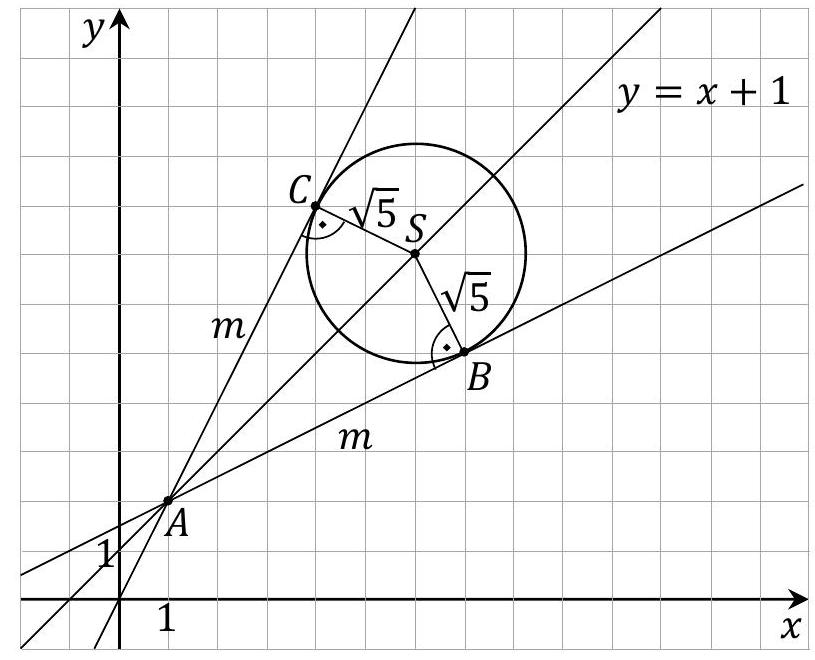
\includegraphics[max width=\textwidth, center]{2025_02_07_d8b842ccd39861fafa8ag-26}

Pole $P_{A B S C}$ czworokąta $A B S C$ jest sumą pól trójkątów przystających $A B S$ oraz $A C S$, więc

$$
\begin{gathered}
P_{A B S C}=P_{A B S}+P_{A C S} \\
15=2 \cdot \frac{1}{2} \cdot m \cdot \sqrt{5} \\
m=3 \sqrt{5}
\end{gathered}
$$

Z twierdzenia Pitagorasa zastosowanego do trójkąta $A B S$ otrzymujemy

$$
|A S|^{2}=|A B|^{2}+|B S|^{2}=(3 \sqrt{5})^{2}+(\sqrt{5})^{2}=50
$$

Niech $x_{S}$ będzie pierwszą współrzędną punktu $S$. Punkt $S$ leży na prostej o równaniu $y=x+1$, więc $S=\left(x_{S}, x_{S}+1\right)$.\\
Wtedy

$$
\left(x_{S}-1\right)^{2}+\left(x_{S}+1-2\right)^{2}=50
$$

Stąd dalej otrzymujemy

$$
\left(x_{S}-1\right)^{2}=25
$$

$$
\begin{gathered}
\left|x_{S}-1\right|=5 \\
x_{S}=6 \vee \quad x_{S}=-4
\end{gathered}
$$

Zatem $S=(6,7)$ lub $S=(-4,-3)$.

\section*{Sposób II}
Promienie $B S$ oraz CS okręgu poprowadzone do punktów styczności są prostopadłe do stycznych - odpowiednio - $A B$ i $A C$, więc trójkąty $A B S$ oraz $A C S$ są prostokątne. Ponadto odcinki $A B$ oraz $A C$ mają równe długości, więc trójkąty te są przystające (na podstawie cechy bbb przystawania trójkątów). Oznaczmy $m=|A B|=|A C|$ (zobacz rysunek).\\
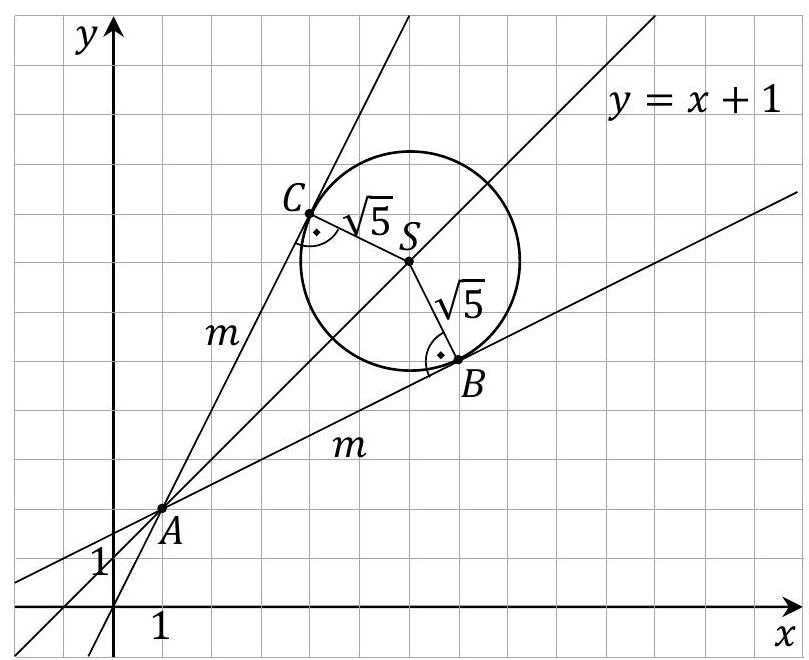
\includegraphics[max width=\textwidth, center]{2025_02_07_d8b842ccd39861fafa8ag-27}

Pole $P_{A B S C}$ czworokąta $A B S C$ jest sumą pól trójkątów przystających $A B S$ oraz $A C S$, więc

$$
\begin{gathered}
P_{A B S C}=P_{A B S}+P_{A C S} \\
15=2 \cdot \frac{1}{2} \cdot m \cdot \sqrt{5} \\
m=3 \sqrt{5}
\end{gathered}
$$

Niech $x_{S}$ będzie pierwszą współrzędną punktu $S$. Punkt $S$ leży na prostej o równaniu $y=x+1$, więc $S=\left(x_{S}, x_{S}+1\right)$.\\
Zauważmy, że punkt $A$ leży na prostej o równaniu $y=x+1$. Każda prosta przechodząca przez punkt $A=(1,2)$, poza prostą równoległą do osi $O y$, ma równanie postaci $y=a(x-1)+2$. Tangens kąta, jaki tworzy każda ze stycznych $A B$ oraz $A C$ z prostą o równaniu $y=x+1$, jest równy

$$
\operatorname{tg} \alpha=\frac{\sqrt{5}}{m}=\frac{\sqrt{5}}{3 \sqrt{5}}=\frac{1}{3}
$$

Stąd i ze wzoru na tangens kąta między prostymi otrzymujemy

$$
\begin{aligned}
& \frac{1}{3}=\operatorname{tg} \alpha=\left|\frac{a-1}{a+1}\right| \\
& a+1=3(a-1) \vee \quad a+1=-3(a-1) \\
& a=2 \quad \vee \quad a=\frac{1}{2}
\end{aligned}
$$

Zatem styczne $A B$ oraz $A C$ mają równania postaci $y=2(x-1)+2$ oraz $y=\frac{1}{2}(x-1)+2$, czyli $2 x-y=0$ oraz $x-2 y+3=0$.\\
Odległość punktu $S$ od każdej ze stycznych $A B$ i $A C$ jest równa $\sqrt{5}$. Zatem

$$
\begin{gathered}
\frac{\left|2 x_{S}-\left(x_{S}+1\right)\right|}{\sqrt{2^{2}+(-1)^{2}}}=\sqrt{5} \\
\left|x_{S}-1\right|=5 \\
x_{S}=6 \quad \vee \quad x_{S}=-4
\end{gathered}
$$

Istnieją dwa punkty spełniające warunki zadania: $S=(6,7)$ oraz $S=(-4,-3)$.

Zadanie 15. (0-6)

\begin{center}
\begin{tabular}{|l|l|}
\hline
\multicolumn{2}{|c|}{Wymagania egzaminacyjne 2024} \\
\hline
\multicolumn{1}{|c|}{Wymaganie ogólne} & \multicolumn{1}{|c|}{Wymagania szczegółowe} \\
\hline
III. Modelowanie matematyczne. & Zdający: \\
 & 3.1R) stosuje wzory Viète'a; \\
 & 3.2R) rozwiązuje równania i nierówności \\
 & liniowe i kwadratowe z parametrem. \\
\hline
\end{tabular}
\end{center}

\section*{Zasady oceniania}
Rozwiązanie zadania składa się z trzech etapów.\\
Pierwszy etap polega na rozwiązaniu nierówności $\Delta>0$. Za poprawne wykonanie tego etapu zdający otrzymuje 1 punkt.\\
1 pkt - poprawne rozwiązanie nierówności $\Delta>0: m \in(-\infty,-3) \cup(1,+\infty)$.\\
0 pkt - rozwiązanie, w którym zastosowano niepoprawną metodę, albo brak rozwiązania.

\section*{Uwaga:}
Jeżeli zdający rozwiązuje warunek $\Delta \geq 0$, to za tę część rozwiązania otrzymuje $\mathbf{0}$ punktów.\\
Drugi etap polega na wyznaczeniu tych wartości parametru $m$, dla których jest spełniony warunek $x_{1}^{3}+x_{2}^{3}+3 \cdot x_{1} \cdot x_{2} \cdot\left(x_{1}+x_{2}-3\right) \leq 3 m-7$. Za poprawne wykonanie tego etapu zdający otrzymuje 4 punkty.\\
Podział punktów za drugi etap rozwiązania:\\
4 pkt - rozwiązanie nierówności $z$ jedną niewiadomą $m$ równoważnej warunkowi

$$
x_{1}^{3}+x_{2}^{3}+3 \cdot x_{1} \cdot x_{2} \cdot\left(x_{1}+x_{2}-3\right) \leq 3 m-7: m \in\left(-\infty, \frac{1}{3}\right) .
$$

3 pkt - zapisanie nierówności z jedną niewiadomą $m$ równoważnej warunkowi\\
$x_{1}^{3}+x_{2}^{3}+3 \cdot x_{1} \cdot x_{2} \cdot\left(x_{1}+x_{2}-3\right) \leq 3 m-7$ w postaci $W(m) \leq 0$, gdzie $W(m)$\\
jest iloczynem co najmniej dwóch wielomianów stopni dodatnich, np .\\
$(3 m-1)(3 m+1)^{2} \leq 0,\left(9 m^{2}-1\right)(3 m+1) \leq 0,27\left(m-\frac{1}{3}\right)\left(m+\frac{1}{3}\right)^{2} \leq 0$\\
ALBO

\begin{itemize}
  \item zapisanie nierówności $z$ jedną niewiadomą $m$ równoważnej warunkowi $x_{1}^{3}+x_{2}^{3}+3 \cdot x_{1} \cdot x_{2} \cdot\left(x_{1}+x_{2}-3\right) \leq 3 m-7 \mathrm{w}$ postaci\\
$27 m^{3}+9 m^{2}-3 m-1 \leq 0$ oraz wyznaczenie jednego $z$ pierwiastków wielomianu $27 m^{3}+9 m^{2}-3 m-1$.\\
2 pkt - zapisanie nierówności z jedną niewiadomą $m$ równoważnej warunkowi\\
$x_{1}^{3}+x_{2}^{3}+3 \cdot x_{1} \cdot x_{2} \cdot\left(x_{1}+x_{2}-3\right) \leq 3 m-7, \mathrm{np}$.\\
$(3 m+1)^{3}-9 \cdot\left(2 m^{2}+m+1\right) \leq 3 m-7$.\\
1 pkt - przekształcenie nierówności $x_{1}^{3}+x_{2}^{3}+3 \cdot x_{1} \cdot x_{2} \cdot\left(x_{1}+x_{2}-3\right) \leq 3 m-7$ do postaci pozwalającej na bezpośrednie zastosowanie wzorów Viète'a, np.\\
$\left(x_{1}+x_{2}\right)^{3}-9 x_{1} x_{2} \leq 3 m-7$.\\
0 pkt - rozwiązanie, w którym zastosowano niepoprawną metodę, albo brak rozwiązania.
\end{itemize}

Trzeci etap polega na wyznaczeniu wszystkich wartości parametru $m$, które spełniają jednocześnie dwa warunki: $\Delta>0$ i $x_{1}^{3}+x_{2}^{3}+3 \cdot x_{1} \cdot x_{2} \cdot\left(x_{1}+x_{2}-3\right) \leq 3 m-7$ : $m \in(-\infty,-3)$.\\
Za poprawne wykonanie tego etapu zdający otrzymuje 1 punkt.\\
1 pkt - poprawne wyznaczenie wszystkich wartości parametru $m$, które spełniają\\
jednocześnie warunki $\Delta>0$ i $x_{1}^{3}+x_{2}^{3}+3 \cdot x_{1} \cdot x_{2} \cdot\left(x_{1}+x_{2}-3\right) \leq 3 m-7$ : $m \in(-\infty,-3)$.\\
0 pkt - rozwiązanie, w którym zastosowano niepoprawną metodę, albo brak rozwiązania.

\section*{Uwagi:}
\begin{enumerate}
  \item Jeżeli zdający w etapie I lub II popełni błąd, który nie jest błędem rachunkowym, to za III etap otrzymuje 0 punktów.
  \item Jeżeli zdający w etapach Ii ll nie popełni błędów innych niż rachunkowe i otrzyma zbiory rozwiązań, które nie są rozłączne i żaden z nich nie jest zbiorem liczb rzeczywistych, a następnie poprawnie wyznaczy część wspólną zbiorów rozwiązań z etapów I i II, to za III etap może otrzymać 1 punkt.
  \item Jeżeli zdający w II etapie rozwiązania popełni błąd - przyjmie, że\\
$x_{1}+x_{2}= \pm\left(2 m^{2}+m+1\right)$ lub $x_{1} \cdot x_{2}= \pm(3 m+1)$, lub $x_{1}+x_{2}= \pm \frac{b}{2 a}$, to za II etap może otrzymać co najwyżej 2 punkty ( 1 punkt za przekształcenie nierówności $x_{1}^{3}+x_{2}^{3}+3 \cdot x_{1} \cdot x_{2} \cdot\left(x_{1}+x_{2}-3\right) \leq 3 m-7$ do postaci pozwalającej na bezpośrednie zastosowanie wzorów Viète'a oraz 1 punkt za konsekwentne rozwiązanie nierówności do końca), a za III etap otrzymuje 0 punktów.
  \item Jeżeli zdający w II etapie rozwiązania popełni błąd, który nie jest rachunkowy, np.:
\end{enumerate}

\begin{itemize}
  \item pominie istotne nawiasy przy przekształcaniu nierówności $x_{1}^{3}+x_{2}^{3}+3 \cdot x_{1} \cdot x_{2} \cdot\left(x_{1}+x_{2}-3\right) \leq 3 m-7$ do postaci pozwalającej na bezpośrednie zastosowanie wzorów Viète'a,
  \item przyjmie, że\\
$x_{1}^{3}+x_{2}^{3}=\left(x_{1}+x_{2}\right)\left[\left(x_{1}+x_{2}\right)^{2}-x_{1} \cdot x_{2}\right]$,
  \item przyjmie, że\\
$x_{1}^{3}+x_{2}^{3}=\left(x_{1}+x_{2}\right)^{3}$,\\
i konsekwentnie do popełnionego błędu doprowadzi rozwiązanie II etapu zadania do końca, to może uzyskać co najwyżej 2 punkty za II etap (1 punkt za zastosowanie wzorów Viète'a oraz 1 punkt za konsekwentne rozwiązanie nierówności do końca), a za III etap otrzymuje 0 punktów.
\end{itemize}

\begin{enumerate}
  \setcounter{enumi}{4}
  \item Jeżeli w II etapie rozwiązania zdający popełni błędy i otrzyma nierówność $V(m) \leq 0$, to za podanie zbioru rozwiązań nierówności otrzymuje 1 punkt tylko wtedy, gdy wielomian $V$ jest stopnia trzeciego i ma co najmniej dwa różne pierwiastki rzeczywiste.
  \item Jeżeli zdający wprowadza dodatkowe założenie, które nie wynika $z$ warunków zadania (np. $x_{1}+x_{2}>0, x_{1} \cdot x_{2}>0$ ), to za całe rozwiązanie może otrzymać co najwyżej 5 punktów (co najwyżej 1 punkt za I etap i co najwyżej 4 punkty za II etap).
\end{enumerate}

\section*{Przykładowe pełne rozwiązanie I etap}
Trójmian kwadratowy $x^{2}-(3 m+1) x+2 m^{2}+m+1$ ma dwa różne pierwiastki rzeczywiste wtedy i tylko wtedy, gdy wyróżnik tego trójmianu jest dodatni. Rozwiązujemy warunek $\Delta>0$ :

$$
\begin{gathered}
{[-(3 m+1)]^{2}-4 \cdot 1 \cdot\left(2 m^{2}+m+1\right)>0} \\
m^{2}+2 m-3>0 \\
(m-1) \cdot(m+3)>0 \\
m \in(-\infty,-3) \cup(1,+\infty)
\end{gathered}
$$

\section*{II etap}
Wyznaczamy wszystkie wartości parametru $m$, dla których jest spełniony warunek $x_{1}^{3}+x_{2}^{3}+3 \cdot x_{1} \cdot x_{2} \cdot\left(x_{1}+x_{2}-3\right) \leq 3 m-7$, korzystając ze wzorów Viète'a:

$$
\begin{gathered}
x_{1}^{3}+x_{2}^{3}+3 \cdot x_{1} \cdot x_{2} \cdot\left(x_{1}+x_{2}-3\right) \leq 3 m-7 \\
\left(x_{1}+x_{2}\right)^{3}-9 x_{1} x_{2} \leq 3 m-7 \\
(3 m+1)^{3}-9 \cdot\left(2 m^{2}+m+1\right) \leq 3 m-7 \\
27 m^{3}+9 m^{2}-3 m-1 \leq 0 \\
(3 m)^{3}-1^{3}+9 m^{2}-3 m \leq 0 \\
(3 m-1)\left(9 m^{2}+3 m+1\right)+3 m(3 m-1) \leq 0 \\
(3 m-1)\left(9 m^{2}+6 m+1\right) \leq 0 \\
(3 m-1)(3 m+1)^{2} \leq 0 \\
m \in\left(-\infty, \frac{1}{3}\right)
\end{gathered}
$$

\section*{III etap}
Wyznaczamy wszystkie wartości parametru $m$, które jednocześnie spełniają warunki $m \in(-\infty,-3) \cup(1,+\infty)$ oraz $m \in\left(-\infty, \frac{1}{3}\right): m \in(-\infty,-3)$.

Zadanie 16. (0-6)

\begin{center}
\begin{tabular}{|l|l|}
\hline
\multicolumn{2}{|c|}{Wymagania egzaminacyjne 2024} \\
\hline
\multicolumn{1}{|c|}{Wymaganie ogólne} & \multicolumn{1}{|c|}{Wymaganie szczegółowe} \\
\hline
III. Modelowanie matematyczne. & Zdający: \\
 & 11.6R) stosuje pochodne do rozwiązywania \\
 & zagadnień optymalizacyjnych. \\
\hline
\end{tabular}
\end{center}

\section*{Zasady oceniania}
\section*{Część a)}
2 pkt - przeprowadzenie pełnego rozumowania.\\
1 pkt - wyznaczenie wysokości $H$ graniastosłupa w zależności od długości krawędzi podstawy, np. $H=\frac{13824}{a^{2} \sqrt{3}}$.\\
0 pkt - rozwiązanie, w którym zastosowano niepoprawną metodę, albo brak rozwiązania.

\section*{Uwagi:}
\begin{enumerate}
  \item Jeżeli zdający rozważa inną bryłę niż graniastosłup prawidłowy trójkątny, to otrzymuje 0 punktów za całe rozwiązanie.
  \item Jeżeli zdający przeprowadzi rozumowanie tylko dla $a=8 \sqrt{3}$, to otrzymuje 0 punktów za całe rozwiązanie części a).
\end{enumerate}

\section*{Część b)}
4 pkt - uzasadnienie, że funkcja $P$ przyjmuje wartość najmniejszą dla $a=8 \sqrt{3}$\\
i obliczenie wartości najmniejszej funkcji $P: 96 \sqrt{3}+1728$.\\
3 pkt - uzasadnienie (np. poprzez badanie monotoniczności funkcji), że funkcja $P$ przyjmuje wartość najmniejszą dla $a=8 \sqrt{3}$\\
ALBO

\begin{itemize}
  \item zapisanie, że dla $a=8 \sqrt{3}$ funkcja $P$ osiąga wartość najmniejszą i obliczenie\\
$P(8 \sqrt{3}): P(8 \sqrt{3})=96 \sqrt{3}+1728$.\\
2 pkt - poprawne rozwiązanie równania $a \sqrt{3}-\frac{13824 \sqrt{3}}{a^{2}}=0: a=24$.\\
1 pkt - wyznaczenie pochodnej funkcji $P: P^{\prime}(a)=a \sqrt{3}-\frac{13824 \sqrt{3}}{a^{2}}$.\\
0 pkt - rozwiązanie, w którym zastosowano niepoprawną metodę, albo brak rozwiązania.
\end{itemize}

\section*{Uwagi do części b):}
\begin{enumerate}
  \item Jeżeli zdający wyznaczy pochodną funkcji $P$ z błędem, ale wyznaczona pochodna ma postać $A a+\frac{B}{a^{2}}$, gdzie $A$ oraz $B$ są liczbami niewymiernymi, lub postać ułamka, $w$ którego liczniku jest wielomian stopnia trzeciego, a w mianowniku $m a^{2}$, i konsekwentnie rozwiąże zadanie do końca, to może otrzymać co najwyżej 3 punkty za całe rozwiązanie części b) (za miejsce zerowe pochodnej, za uzasadnienie istnienia najmniejszej wartości funkcji oraz za obliczenie najmniejszej wartości funkcji $P$ ).
\end{enumerate}

Jeżeli natomiast otrzyma inną błędną postać pochodnej, to może otrzymać co najwyżej 2 punkty za całe rozwiązanie części b) (za miejsce zerowe pochodnej oraz za uzasadnienie istnienia najmniejszej wartości funkcji $P$ ).\\
2. Badanie znaku pochodnej zdający może opisać w inny sposób, np. szkicując wykres funkcji, która w ten sam sposób jak pochodna zmienia znak, i zaznaczając na rysunku, np. znakami „,"" i ,"" znak pochodnej.\\
3. Jeżeli zdający otrzyma miejsce zerowe pochodnej, które należy do przedziału $(0,8 \sqrt{3})$, to może otrzymać za część b) co najwyżej 1 punkt (za wyznaczenie pochodnej albo za obliczenie miejsca zerowego pochodnej).\\
4. Za poprawne uzasadnienie, że funkcja $P$ osiąga wartość najmniejszą dla $a=8 \sqrt{3}$ można uznać sytuację, gdy zdający bada znak pochodnej oraz zapisuje słownie lub graficznie, że funkcja $P$ jest malejąca w przedziale ( $0, a_{0}$ ), gdzie $a_{0}$ jest miejscem zerowym pochodnej funkcji $f$, będącej rozszerzeniem funkcji $P$ na zbiór $(0,+\infty)$.\\
5. Jeżeli zdający błędnie uzasadnia, że dla $a=8 \sqrt{3}$ funkcja $P$ osiąga wartość najmniejszą, to nie otrzymuje punktu za obliczenie $P(8 \sqrt{3})$.

\section*{Przykładowe pełne rozwiązanie}
\section*{a)}
Rozpatrzmy dowolny z rozważanych graniastosłupów. Oznaczmy jego wysokość przez H. Korzystamy ze wzoru na objętość graniastosłupa oraz wzoru na pole trójkąta równobocznego i otrzymujemy:

$$
\begin{gathered}
3456=\frac{a^{2} \sqrt{3}}{4} \cdot H \\
H=\frac{4608 \sqrt{3}}{a^{2}}
\end{gathered}
$$

Stąd oraz ze wzoru na pole powierzchni całkowitej graniastosłupa dostajemy

$$
\begin{gathered}
P=2 \cdot \frac{a^{2} \sqrt{3}}{4}+3 a H \\
P=\frac{a^{2} \sqrt{3}}{2}+3 a \cdot \frac{4608 \sqrt{3}}{a^{2}} \\
P(a)=\frac{a^{2} \sqrt{3}}{2}+\frac{13824 \sqrt{3}}{a}
\end{gathered}
$$

b)

Obliczamy najmniejszą wartość funkcji $P$ określonej wzorem $P(a)=\frac{a^{2} \sqrt{3}}{2}+\frac{13824 \sqrt{3}}{a}$ dla $a \in(0,8 \sqrt{3}\rangle$.\\
Wyznaczamy pochodną funkcji $P: P^{\prime}(a)=a \sqrt{3}-\frac{13824 \sqrt{3}}{a^{2}}$ dla $a \in(0,8 \sqrt{3}\rangle$.

Obliczamy miejsca zerowe pochodnej funkcji $P$ :

$$
\begin{gathered}
P^{\prime}(a)=0 \\
a \sqrt{3}-\frac{13824 \sqrt{3}}{a^{2}}=0 \\
a^{3} \sqrt{3}-13824 \sqrt{3}=0 \\
a^{3}=13824=24^{3} \\
a=24 \notin(0,8 \sqrt{3}\rangle
\end{gathered}
$$

Badamy znak pochodnej:

$$
\begin{gathered}
P^{\prime}(a)<0 \\
a \sqrt{3}-\frac{13824 \sqrt{3}}{a^{2}}<0 \\
a^{3} \sqrt{3}-13824 \sqrt{3}<0 \\
a^{3}<13824 \\
a<24
\end{gathered}
$$

więc $P^{\prime}(a)<0$ dla $a \in(0,8 \sqrt{3}\rangle$.\\
Zatem funkcja $P$ jest malejąca w przedziale ( $0,8 \sqrt{3}\rangle$.\\
Stąd dla $a=8 \sqrt{3}$ funkcja $P$ osiąga wartość najmniejszą równą\\
$P(8 \sqrt{3})=\frac{a^{2} \sqrt{3}}{2}+\frac{13824 \sqrt{3}}{a}=\frac{(8 \sqrt{3})^{2} \cdot \sqrt{3}}{2}+\frac{13824 \sqrt{3}}{8 \sqrt{3}}=96 \sqrt{3}+1728$.


\end{document}